\subsection{Computational Fracture Mechanics}

The stress intensity factors used in this research were simulated using finite element analysis, with the software tools FRANC3D and Abaqus \cite{f3d, Abaqus}. Abaqus served as the primary tool for creating and solving the finite element mesh. FRANC3D was employed for tasks related to crack insertion and SIF computation. Abaqus Python was used to generate the model geometries.

For increased reliability in crack insertion using FRANC3D, a local-global sub-modeling approach was employed. This method involved dividing the geometry into two components: the global model, which encompassed the boundary conditions, and the local model, focused on the region where the crack would be inserted. The local model is used in FRANC3d, where the crack is inserted using rings of hexagonal elements, with an inner ring of quarter-point elements surrounding the crack front, allowing for SIF calculations (as shown in Figure \ref{fig:f3d_mesh}). The remainder of the local model was re-meshed, preserving the nodal locations around the cut faces for later reattachment to the global model. The recombined model with the inserted crack was subsequently solved using the Abaqus solver. This process is illustrated in \ref{fig:f3d_abq_flow}.



\begin{figure}
  \centering
  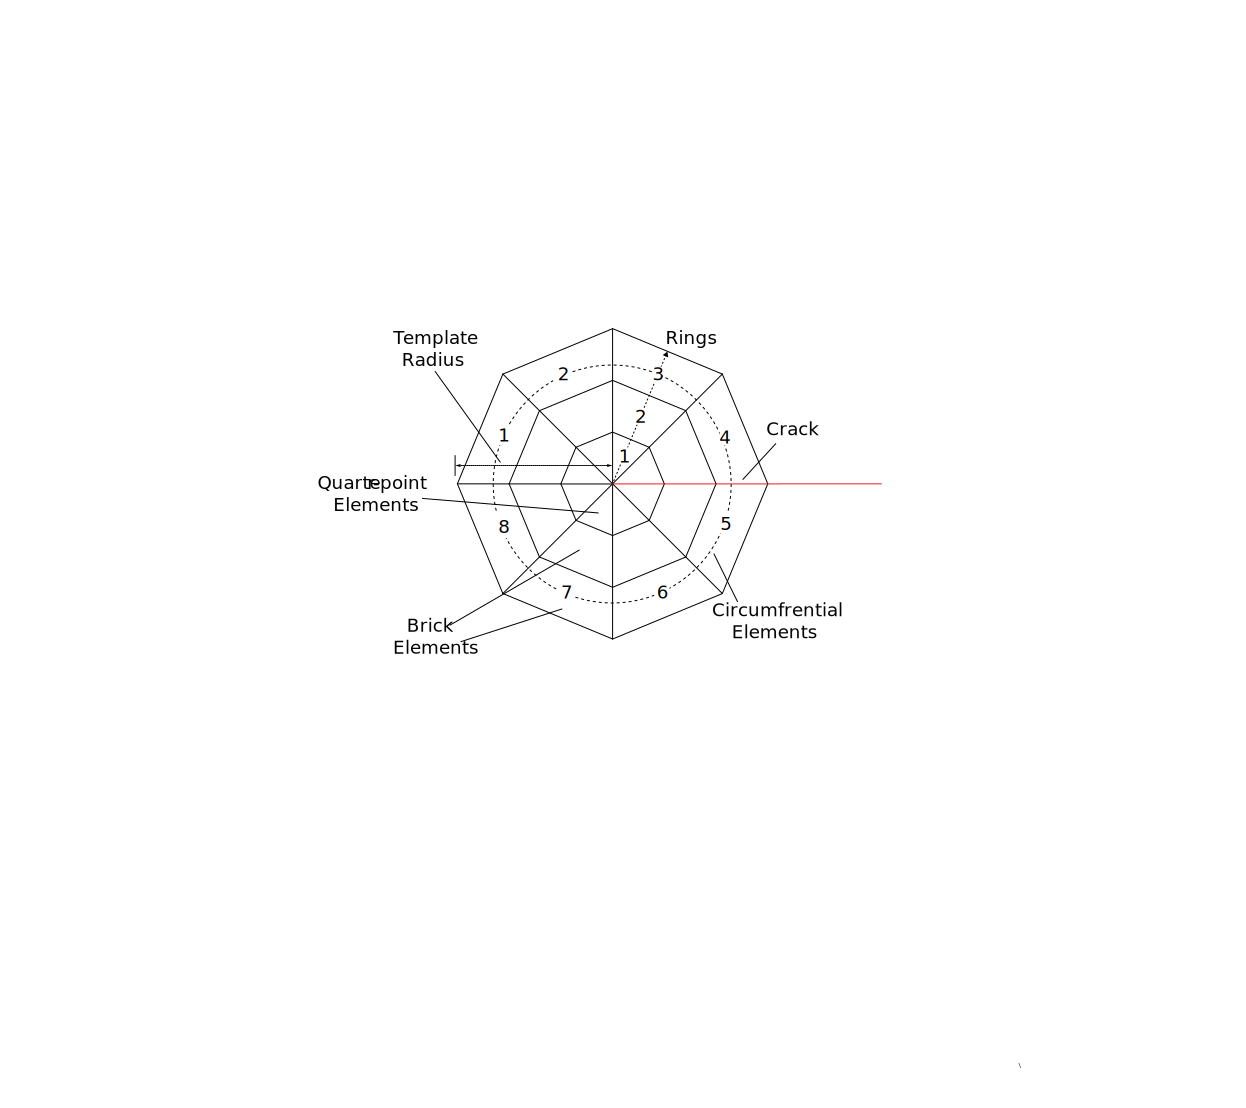
\includegraphics[width=0.8\textwidth]{geometry_figures/f3d_crack.png}
  \label{fig:f3d_crack}
  \caption{FRANC3D crack mesh containing 8 circumferential elements and 3 rings. The template radius is the radius of an inscribed circle}
\end{figure}

Integral methods are preferred over displacement methods, such as displacement correlation, for the caluculation of SIFs. Integral methods assess the energy of the cracked system, providing greater accuracy. The J-integral, developed by \cite{Rice1968}, is a commonly used method for SIF calculation. However, it has a limitation - it cannot separate the SIFs into the three cracking modes, except for very simplified crack geometries, as noted by \cite{Banks-Sills2005}.

To address this limitation, the M-integral offers a solution by using a combination of two SIFs: one representing the true SIF and the other an arbitrary solution. By employing this approach, it becomes possible to extract each SIF corresponding to the three cracking modes, as explained by \cite{Banks-Sills2005}. The M-integral is defined as follows:

\begin{equation}\label{eqn:M-Integral}
    M^{(1, 2)} = \int_\Gamma \left(W^{(1,2)}n_1 - T^{(1)}_i \frac{\partial u^{(2)}_i}{\partial x_1} - T^{(2)}_i \frac{\partial u^{(1)}_i}{\partial x_1} \right) \, \text{d}s,
\end{equation}

Here, $T_i = \sigma_{ij} n_j$ represents the traction vector, $W = 1/2 \sigma_{ij} \epsilon_{ij}$ stands for the strain energy density, and the superscripts 1 and 2 correspond to the two superposed solutions.


\subsection{Genetic Programming Based Symbolic Regression}
% look at previous papers to write this Karl, Donovan, Geoff plasticity paper
% https://arxiv.org/abs/2304.01117

Symbolic Regression (SR) is a machine learning technique aimed at discovering closed-form analytical expressions that accurately fit training data. Presently, the most effective optimization approach for SR is genetic programming (GP) \cite{GPSR-comp}. The implementation of genetic programming based symbolic regression (GPSR) employed in this research is an open-source Python package known as Bingo \cite{Randall2022}. Bingo, enables the learning of real-valued mathematical expressions represented as acyclic graphs (Agraphs) enabling adaptive adjustments throughout training. The equation's complexity is determined by the number of nodes in the Agraph, figure \ref{fig:agraph} shows an Agraph for the equation $C_0 X_0 + C_1 X_1$, that has a complexity of 7 corresponding to the 7 nodes in the Agraph. The training begins with an initial assortment of randomly generated equations, varying in complexity. During each generation, equations undergo randomized modifications, employing a combination of crossover and mutation. Crossover entails selecting nodes from two Agraphs and exchanging these nodes along with their associated branches and leaves, generating two new equations. Mutation, on the other hand, introduces random changes to nodes in the Agraph as shown in figure \ref{fig:agraph_cross_mut} \cite{Schmidt2007}. After crossover and mutation has occurred the equations are ranked based on a defined fitness criterion, a user-set function that heavily influences the algorithm's speed and results. The best equations are then used in the next generation where the cycle continues until a fitness threshold or maximum number of generations has been satisfied. 

\begin{figure}
    \centering
    \includegraphics[width=0.6\textwidth]{geometry_figures/agraph.png}
    \label{fig:agraph}
    \caption{Example Agraph for for equation; $C_0 X_0 + C_1 X_1$, where the complexity is the sum of the nodes in this case 7.} 
\end{figure}


\begin{figure}
    \centering

    \begin{minipage}{\textwidth}
        \centering
        \includegraphics[width=0.8\linewidth]{geometry_figures/agraph-crossover.png}
        \caption*{(a)}
    \end{minipage}
    
    \begin{minipage}{\textwidth}
        \centering
        \includegraphics[width=0.8\linewidth]{geometry_figures/agraph-mutation.png}
        \caption*{(b)}
    \end{minipage}
    
    \caption{(a) crossover, where two parent graphs combine features to create a child graph. (b) where part of a graph is randomly changed creating a new graph.}
    \label{fig:agraph_cross_mut}
\end{figure}




The best performing equations according to the fitness metric from the final population are taken and presented as a Pareto front figure \ref{fig:perato-front} where both the complexity and fitness of each equation can be visualized. Because GPSR is an interpretable ML method, intepretability of the chosen equation is often important. Equations with high complexity have better fitness values; however, they can lack interpretabiliy. Equations with low complexity tend to be easily interpreteble at the expense of decreased fitness. The user must decide what equation is the best for the application. Typically there is a point at which increasing the complexity yields little gain on fitness this optimal value can be seen in Figure \ref{fig:perato-front}. 

\begin{figure}
    \centering
    \includegraphics[width=0.6\textwidth]{Figures/dummy_pareto_front.png}
    \label{fig:perato-front}
    \caption{Example Pareto front where the horizontal axis is the model complexity and the vertical axis is the model fitness. Each point on the graph represents a different model in the population.} 
\end{figure}




 